\chapter{WORKLOAD CHARACTERIZATION}
\label{chap:character}
%
In this section, I characterize mobile workloads for the
suitability of offloading from the perspective of {\it Computation to
Communication ratio} which is calculated by the time for workloads to be
executed locally divided by the data transfer time for the remote
offloading.
%
Thus in this work, computation to communication ratio for each workload is
a comprehensive measurement which mirrors three parameters such as the
volume of computation of workloads, the amount of data to be transferred, and the
network conditions. 
%
As part of the workload characterization effort through computation to
communication ratio, I strategically selected four quantitatively and qualitatively 
different OpenCL workloads for the analysis:
sobelfilter, matrix multiplication, {\it N}-body physics and hidden
Markov model, each being classified into two categories: 
the computation-intensive workload (matrix multiplication and 
{\it N}-body physics) and the communication-intensive workload 
(sobelfilter and hidden Markov model) in terms of computation to communication ratio.
%
Note that though computation- or communication-intensity of
four OpenCL workloads is not absolute, it is worth to categorize 
the relative computation- or communication-intensity of the workloads so
it is possible to explore the workload conditions where offloading is
more beneficial than local processing.\\    
%
Furthermore, I deployed the offloading framework into the
various types of network such as local area networks, campus networks
and Amazon EC2 instance which have different network restrictions, and
set various levels of the computing capability of the remote
resource from general purpose CPUs to Amazon EC2 GPUs cluster instance to
analyze the behavior of the remote offloading framework in terms of the
performance and energy implication of mobile devices in accordance with
environmental factors such as network conditions and the computing
capabilities of offloadable resources.
%
For example, I configure local area networks by directly connecting a
mobile device and a remote resource with NVIDIA graphics processing
units via a wireless router which represents the best resource of our
experimental setups.
%
The experimental results show that although not all types of workloads
benefit from mobile workload offloading, there clearly exist a class of
workloads and environmental conditions that can leverage the remote
offloading.
%
\section{Related Works}
\label{character:relatedworks}
In~\cite{fullsystem}, the authors characterize the microarchitectural
behavior of smartphone applications through several representative
benchmarks including the following areas: an interactive game, a
streaming player and mp3 audio player.
%
Also, they developed a new benchmark to characterize the performance 
of a web browser called BBench.
%
Through those benchmarks, they show how they differ from SPEC CPU2006
benchmarks which are widely used for the measurement of compute-intensive
performance.
%
MEVBench~\cite{mevbench} presented a custom benchmark suite for full mobile
vision applications such as augmented reality as well as components of
common vision algorithms such as SIFT feature extraction and SVM
classification.
%
The authors evaluated the performance of MEVBench with various
platforms for the direction of future mobile embedded vision
architectures.
%
Also, they show that mobile vision architectures require to be supported
from heterogeneous computation for performance improvement.
%
In~\cite{characterization}, the performance and energy benefits of
mobile heterogeneous computing are characterized by using 2D FFT(Fast
Fourier Transformation), matrix multiplication, and 2D Stencil as the
benchmarks.
%
In this study, the authors demonstrated that fully utilizing available
computing cores to complete a task can achieve an 3.7$\times$ speed-up
over the case of the single-threaded CPU, consequently, reduce the
energy consumption for the mobile platform.\\
%
In contrast with the aforementioned studies which designed new
benchmarks or characterized the performance and energy benefits of
the mobile platforms via the various workloads from a perspective of
mobile computing capabilities, I characterized the behavior of mobile
offloading framework while considering the network conditions as well as
the computing capabilities of remote resources.
%
\section{Methodology}
\label{character:methodology}
%
The main contribution of this work is to analyze the behavior of the
remote offloading in accordance with the characteristics of the
workloads and environmental factors such as network conditions and the
level of computing capabilities of remote resources.
%
In this section, I explain the workloads used for the analysis and the
way to characterize the workloads as well as experimental setup.
%
Every experiment is repeated 5 times and the results are the averaged 
values.
%
\subsection{Hardware Setup}
\label{character:setup}
%
In order to analyze the behavior of our remote offloading framework
under the various network conditions and the computing capabilities of
remote resources, I setup the experiment using various hardware and
network configurations.
%
First of all, the hardware setup consists of a client and various types of
remote resources.
%
I have utilized Android tabletPC, Samsung GalaxyTab 10.1 equipped with
1Ghz dual-core process and 1GB RAM, and running Android honeycomb as the
mobile client.
%
I adopted three types of servers: CPU only-installed server,
GPU-installed server, and Amazon EC2 GPU cluster.
%
For CPU only-installed server without a graphics card, I utilized a
workstation with Intel 3.0Ghz Core 2 Duo processor and 8GB memory
installed with Linux OS.
%
Also, I installed GeForce GT 640 graphics card with 2GB RAM for the
server with GPUs.
%
In addition, I used Amazon EC2 GPU cluster resource with two NVIDIA
GPUs equipped with 3GB on-board memory per GPU.\\
%
In order to analyze the impact of network conditions on offloading
performance, I configured both local and wide area networks using
following setup.
%
Firstly, I built a local area network by directly connecting the mobile
client and the server through a wireless router supporting 802.11 b/g/n
network standard.
%
Secondly, I used our campus network in order to configure a wide-area
network in which the client and the server connect to a wireless and
wired network respectively.
%
Also, I emulate different wide-area network conditions between the
client and the server by controlling the network latency using Traffic
Control (TC)~\cite{tc}.
%
TC is a network tool which provides functionalities to control network
traffic by prioritizing network resources and using concepts of traffic
classification, queue disciplines and quality of service(QoS).
%
Furthermore, utilizing an instance of Amazon EC2 GPU cluster gives us
one more option for the server located in wide-area network.
%
Table~\ref{table:network_summary} shows the average and standard deviation of network latency and
bandwidth for our network configurations.
%
\begin{table}
\centering
\caption{Average and standard deviation of network latency and bandwidth
for local and wide area networks including Amazon EC2.}
	\begin{tabular}{c|cc|cc|cc}
	\hline
	\ & \multicolumn{2}{c|}{LAN} & \multicolumn{2}{c|}{Campus network} &
\multicolumn{2}{c}{Amazon EC2} \\
	\hline
	Latency & Avg. & Stdev. & Avg. & Stdev. & Avg. & Stdev.\\
	(\textit{ms}) & 10.833 & 2.684 & 15.465 & 4.189 & 74.036 & 17.737 \\ 
	Bandwidth & Avg. & Stdev. & Avg. & Stdev. & Avg. & Stdev. \\
    (\textit{MB/s}) & 6.523 & 0.177 & 2.461 & 0.238 & 0.178 & 0.023 \\ \hline
	\end{tabular}
\label{table:network_summary}
\end{table}
%
\subsection{OpenCL Workloads}
\label{character:workloads}
%
I utilized OpenCL SDK code samples provided by AMD APP
SDK~\cite{amd} and NVIDIA~\cite{nvidia} to choose appropriate workloads for
the remote offloading framework.
%
In order to choose appropriate OpenCL workloads among a set of samples,
I expected that the more computation- and less communication-intensive
the workloads, the more potential gain from remote offloading.
%
Furthermore, I characterized the workloads in accordance with the
amount of computation and communication for input and output data
transfer by considering computation to communication ratio
calculated by the execution time required to process a certain amount of
data locally divided by the data transfer time for the remote offloading.
%
Thus, computation to communication ratio is a
comprehensive measurement which mirrors three parameters such as the
the volume of computations of workloads, the amount of data to be transferred, and the
network conditions.
%
After careful considerations, I chose four qualitatively and
quantitatively different workloads: sobelfilter, matrix multiplication,
hidden Markov model, and {\it N}-body physics used by a variety of areas such as
image processing, physics simulation, and mathematical modeling.
%
Also, since it is necessary to consider an additional interaction 
between the client and the server such as device configuration 
or state transfer which occurs further overhead for communication, 
I examined the programming flow of the application-layer for each workload.
%
The programming flow and structure of workloads are described in the following:\\
%
{\bf Sobelfilter:} Sobelfilter is an image processing filter used for
image edge detection.
%
It consists of both a 3$\times$3 horizontal and vertical filter.
%
The edge detection process applies two filters into an input image in a
sequence and adds final results to a form of the image.
%
Accordingly, the client transfers the horizontal, vertical filter, and
the input image as states for the execution and sets them as arguments
accessed by the kernel.
%
In the server side, the image is iteratively processed based upon the
filters that the client has sent.
%
Once the execution is completed, the server sends back an output image
into the client.
%
Figure~\ref{fig:program_flow1} shows the program flow diagram for the data transfer, the argument
setup, and the kernel execution for sobelfilter.\\
%
{\bf Matrix multiplication:} Similarly to sobelfilter, the client
sends to floating-point matrices ({\it n} by {\it n} and
{\it n} by {\it 2n}) and additional small states and
arguments necessary for the remote kernel execution.
%
Then, server executes multiplication of two matrices and returns one
{\it n} by {\it 2n} matrix to the client as the result.
%
Therefore, matrix multiplication also follows the program flow of
Figure~\ref{fig:program_flow1}.\\
%
{\bf {\it N}-body physics:} {\it N}-body physics is a
mathematical simulation for predicting a dynamic system consisting of
particles or astronomical objects under physical forces such as gravity.
%
In the OpenCL workload for {\it N}-body physics, the client generates
initial states for a certain number of objects and sends them as an
input data.
%
However, the kernel takes additional arguments for each iteration of
kernel execution incurring additional communication between the client
and the server for the arguments setup.
%
The program flow for {\it N}-body physics is shown in
Figure~\ref{fig:program_flow2}.\\
%
{\bf Hidden Markov model:} Hidden Markov model is a popular
statistical tool for modeling generative sequences which can be
characterized by observable sequences.
%
It has been applied to a wide range of applications such as image,
speech recognition, computational biology, bioinformatics and
environment engineering.
%
The OpenCL workload for hidden Markov model follows similar steps for
kernel execution as \textit{N}-body physics.
%
The client generates and transfers initial states and transition
probabilities to the server.
%
Also, the client sends different arguments in order to execute each
iteration of the kernel.
%
Therefore, the program flow for hidden Markov model is represented by
Figure~\ref{fig:program_flow2}.
%
\begin{figure}
\centering
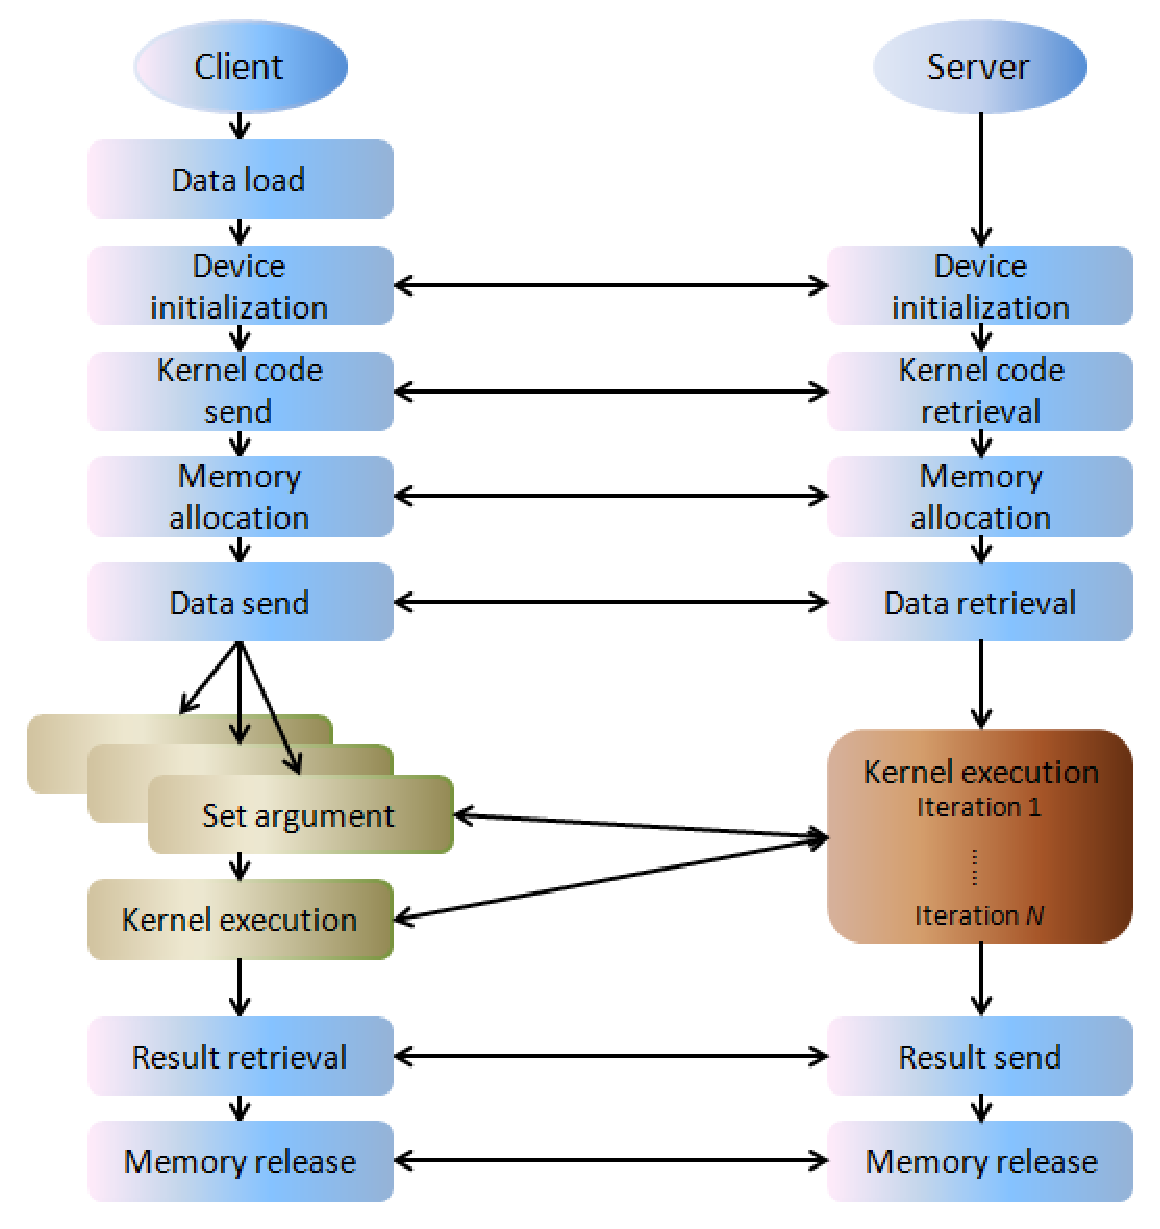
\epsfig{file=figs/program_flow1.eps, width=4.0in}
\caption{Program flow diagram for OpenCL workloads(A)}
\label{fig:program_flow1}
\end{figure}
%
\begin{figure}
\centering
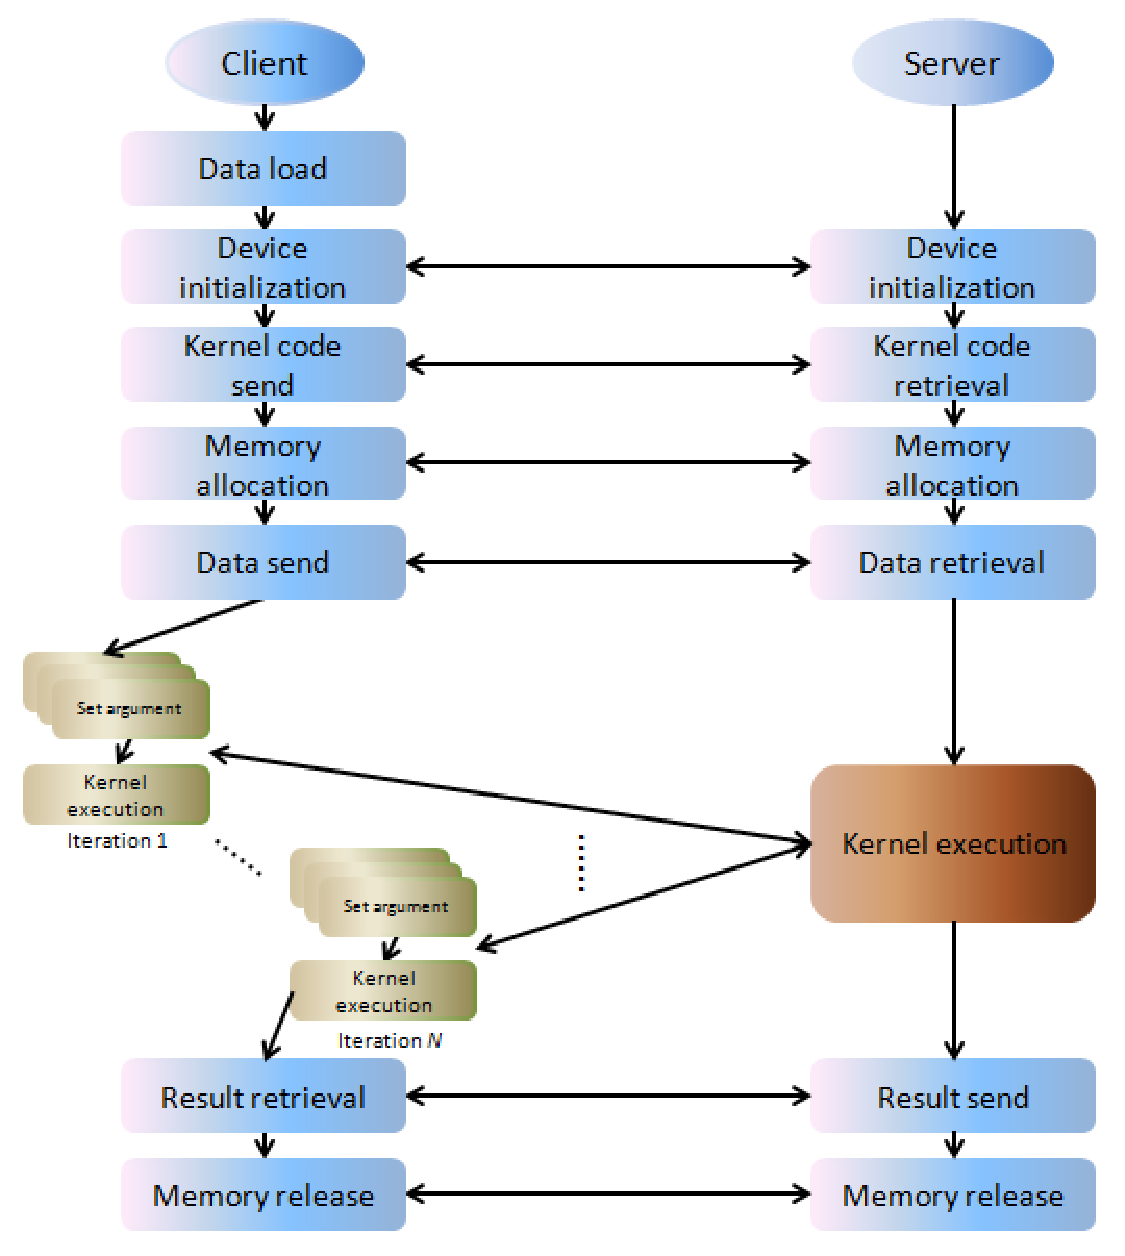
\epsfig{file=figs/program_flow2.eps, width=4.0in}
\caption{Program flow diagram for OpenCL workloads(B)}
\label{fig:program_flow2}
\end{figure}
%
\section{Analysis}
\label{character:analysis}
%
In this section, I analyze the behavior of the OpenCL-based remote
offloading framework for mobile platforms in accordance with the
workload characteristics and environmental factors such as network
conditions and the computing capabilities of remote resources through
real deployment over local and wide area environments.
%
First of all, I observe computation to communication ratios of the
workloads for the given size of data and network configurations.
%
Next, I evaluate the efficacy and the cost of the remote offloading
framework with the various network configurations and the remote
resources.
%
Table~\ref{table:workload_summary_sm} and~\ref{table:workload_summary_hn} 
summarize the amount of input and output data transfer, and the number
of additional API calls for argument setup required to execute the
OpenCL kernel code for the given size of data or the number of
iterations.
%
\begin{landscape}
%\begin{sidewaystable}
\begin{table}
\centering
\caption{Summary of input, output, and number of API calls for
sobelfilter and matrix multiplication}
	\begin{tabular}{c|c|c|c|c|c|c|c|c|c}
	\hline
	 \multicolumn{5}{c|}{Sobelfilter} & \multicolumn{5}{c}{Matrix
multiplication} \\ \hline
	Image size & 480$\times$270 & 960$\times$540 & 1440$\times$810 &
1920$\times$1080 & Matrix size & 160$\times$320 & 400$\times$800 & 560
$\times$1120 & 720$\times$1440 \\
	Input & 390 & 1,520 & 3,310 & 5,790 & Input & 270 & 1,720 & 3,390 & 4,610 \\
	Output & 110 & 370 & 720 & 1,190 & Output & 170 & 1,280 & 2,010 & 3,340 \\
	\# of API calls & 7(0.5) & 7(0.5) & 7(0.5) & 7(0.5) & \# of API calls & 8(0.05) & 8(0.05) & 8(0.05) & 8(0.05) \\ \hline
\end{tabular}
\label{table:workload_summary_sm}
%\end{sidewaystable}
\end{table}
\end{landscape}
%
\begin{landscape}
%\begin{sidewaystable}
\begin{table}
\centering
\caption{Summary of input, output, and number of API calls for
hidden Markov model and N-body physics}
	\begin{tabular}{c|c|c|c|c|c|c|c|c|c}
	\hline
	 \multicolumn{5}{c|}{Hidden Markov model} &
\multicolumn{5}{c}{\textit{N}-body physics} \\ \hline
	number of states & 288 & 640 & 928 & 1,216 & number of iterations &
5 & 10 & 50 & 100 \\ \hline
	Input & 290 & 1,470 & 3,200 & 5,500 & Input & 15 & 15 & 15 & 15 \\
\hline
	Output & 78 & 108 & 110 & 119 & Output & 30 & 30 & 30 & 30 \\ \hline
	\# of API calls & 1000(66) & 1000(66) & 1000(66) & 1000(66) &
\# of API calls & 20(0.16) & 40(0.32) &
200(1.6) & 400(3.2) \\ \hline
\end{tabular}
\label{table:workload_summary_hn}
%\end{sidewaystable}
\end{table}
\end{landscape}
%
\subsection{Computation to Communication Ratio}
\label{character:ctoc}
%
In this section, I present computation to communication ratio 
for each workload for the given size of data and network configurations.
%
As I expected, it is evident that for all workloads, computation to communication
ratio with local area networks is higher than other network
configurations, since the data transfer time becomes shorter by higher
network bandwidth from local area networks.
%
On the contrary to local area networks, the cases of Amazon EC2 have the
lowest computation to communication ratio because of its most restricted
network conditions.
%
As shown in Figure~\ref{fig:ctoc_sobelfilter} and~\ref{fig:ctoc_hmm}, however, 
computation to communication ratios 
for sobelfilter and hidden Markov model are relatively uniform
regardless of the size of data, while those for matrix multiplication
and {\it N}-body physics increase as the size of data or the
number of iterations increases. 
%
This is because that the volume of computations for sobelfilter and
hidden Markov model is linearly proportional to the amount of data to be
processed, while that for matrix multiplication and
{\it N}-body physics increases exponentially as the size of data or
the number of iteration increases, which means that the benefits from
offloading such workloads to more powerful resources also increase exponentially.
%
Therefore, I expect it is highly likely that more gain is available
from offloading matrix multiplication and \textit{N}-body physics 
as the size of data increases. 
%
\begin{figure}
\centering
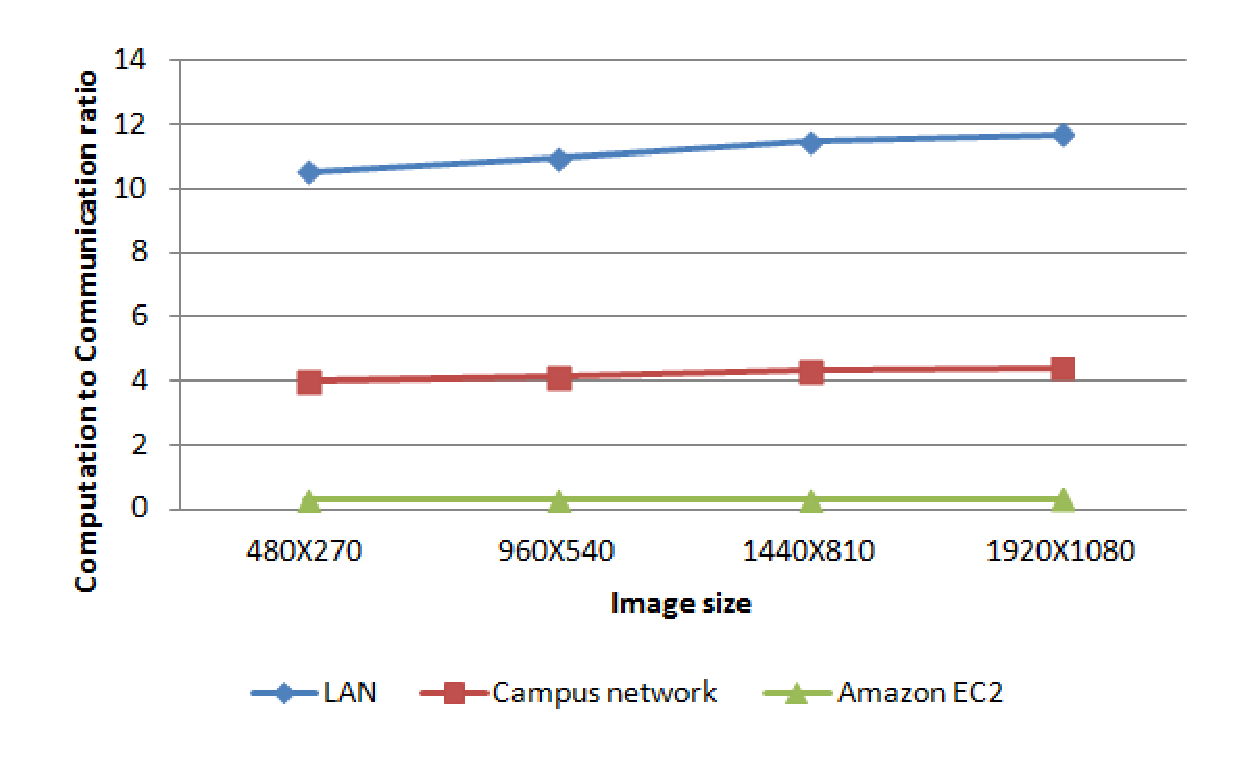
\epsfig{file=figs/ctoc_sobelfilter.eps, width=5.0in}
\caption{Computation to communication ratio for sobelfilter}
\label{fig:ctoc_sobelfilter}
\end{figure}
%
\begin{figure}
\centering
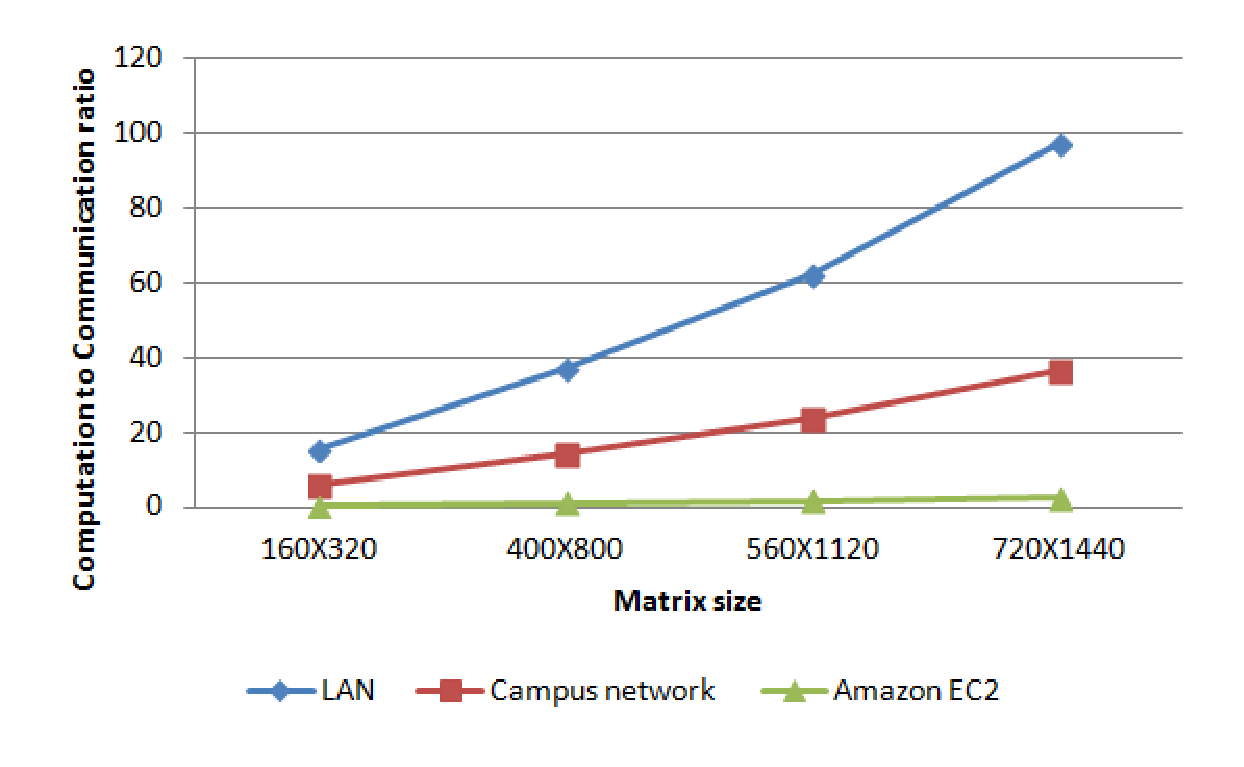
\epsfig{file=figs/ctoc_matrix.eps, width=5.0in}
\caption{Computation to communication ratio for matrix multiplication}
\label{fig:ctoc_matrix}
\end{figure}
%
\begin{figure}
\centering
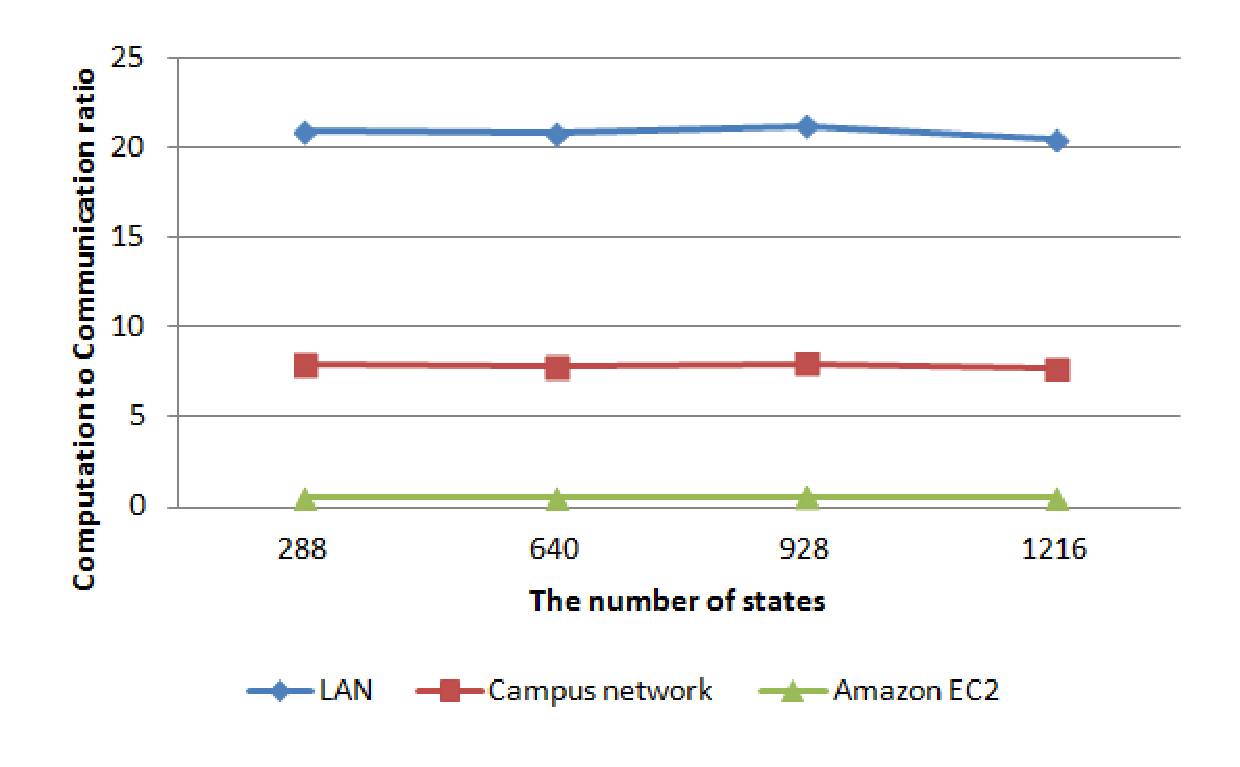
\epsfig{file=figs/ctoc_hmm.eps, width=5.0in}
\caption{Computation to communication ratio for hidden Markov model}
\label{fig:ctoc_hmm}
\end{figure}
%
\begin{figure}
\centering
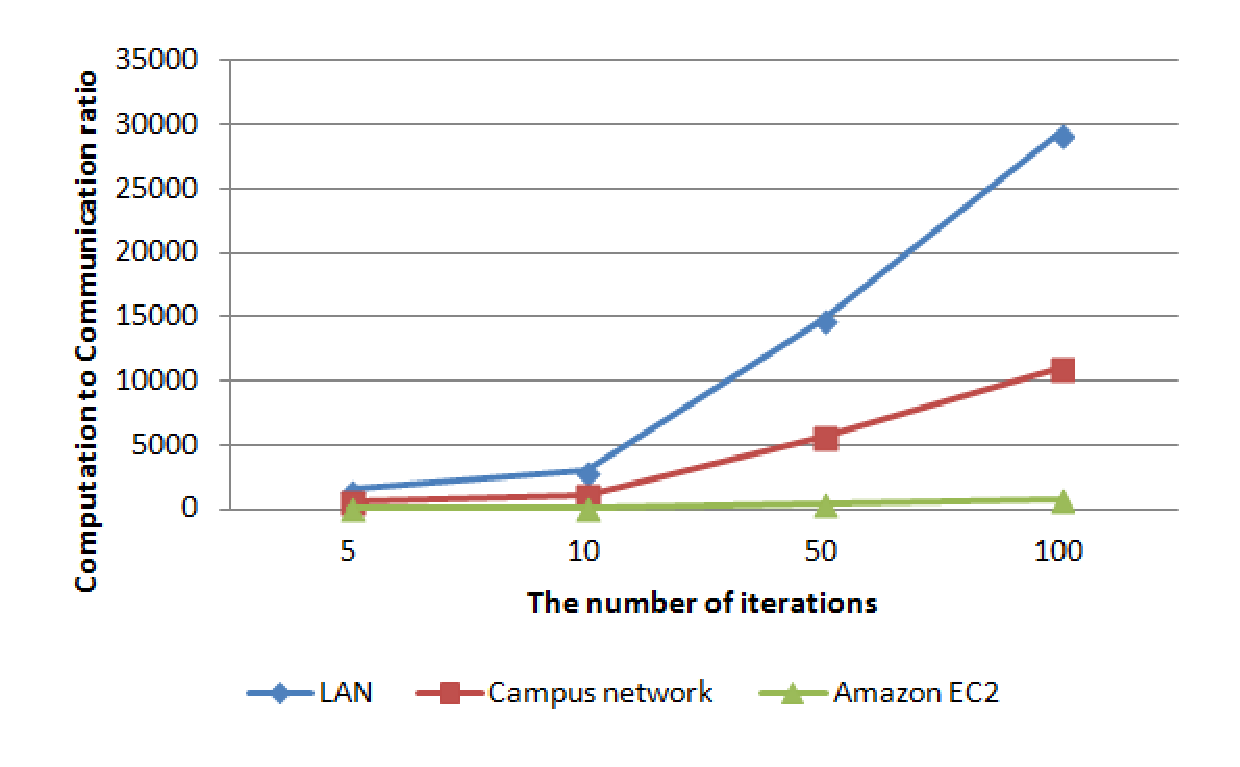
\epsfig{file=figs/ctoc_nbody.eps, width=5.0in}
\caption{Computation to communication ratio for {\it N}-body physics}
\label{fig:ctoc_nbody}
\end{figure}
%
\subsection{Offloading Performance}
\label{character:perf}
%
First of all, for sobelfilter, I observed better performance from
only a few cases where offloading 1440$\times$810 and 1920$\times$1080
of the image size to remote resources located in local area network
than local processing in Figure~\ref{fig:time_sobelfilter}. 
%
In fact, sobelfilter has lower computation to communication
ratios that other workloads ranging from 0.28 to 11.68 in the
experimental setup which indicates it is less computation-intensive 
(i.e. more communication-intensive) workload.
%
Especially, the cases of offloading to the resources located in campus
network and Amazon EC2 cluster instance whose computation to
communication ratio is fairly low have the worst performance in
sobelfilter.  
%
Also, I observed that better performance comes from more powerful
computing power by comparing CPU only-installed server and GPU installed
server in the same network configuration.
%
In contrast to sobelfilter, in all the cases of matrix
multiplication except for 160$\times$320 of matrix size, offloading is
much faster than local processing showing the speed-up which ranges from
1.2$\times$ to 9.2$\times$ as shown in Figure~\ref{fig:time_matrix}.
%
As mentioned in previous section, computation to communication ratios 
of matrix multiplication with the experimental setup range from 0.41 to 97.42 
which means that matrix multiplication is more computation-intensive workload 
than sobelfilter. 
%
Therefore, it is highly likely that matrix multiplication is able to
gain more from offloading to the remote resources with more powerful
computing capabilities.
%
In fact, the computation for matrix multiplication has higher complexity
than sobelfilter (the computation for matrix multiplication is
{\it O}($n^{3}$) while sobelfilter is {\it O}($n^{2}$)).
%
For the smallest matrix size of the setup, 160$\times$320, however,
I observed similar results as 1440$\times$810 and 1920$\times$1080 of
image size in sobelfilter where only offloading to resources in local
area networks has better performance than local processing.
%
With the results of sobelfilter and matrix multiplication, it is evident
that as computation to communication ratio becomes higher, 
it is possible to gain more from offloading.\\
%
Interestingly, in the cases of hidden Markov model, the
extremely worst performance is shown when the workload is offloaded to
Amazon EC2 GPU cluster which has the worst restrictions in terms of
network latency and bandwidth.
%
Though hidden Markov model has higher computation to communication
ratio than sobelfilter, the kernel for hidden Markov model is repeatedly executed 
requiring additional argument setups for each execution which incur 
more communication overhead as described in
section~\ref{character:workloads}.
%
In the Amazon EC2 setup, packets are sent or received at higher
latencies compared to the local area networks which impacts performance
especially since the OpenCL-based offloading framework requires that each RPC call is
acknowledged with a response from the server.
%
Consequently, offloading to Amazon EC2 GPU cluster, which has the
highest latency among the experimental setups, takes the longest time.
%
However, though {\it N}-body physics has the similar programming flow
as hidden Markov model, all the cases of offloading have better
performance than local processing because it is the most
computation-intensive workload among the experimental setup whose
computation to communication ratios range from 40.36 to 29323.68. 
%
\begin{figure}
\centering
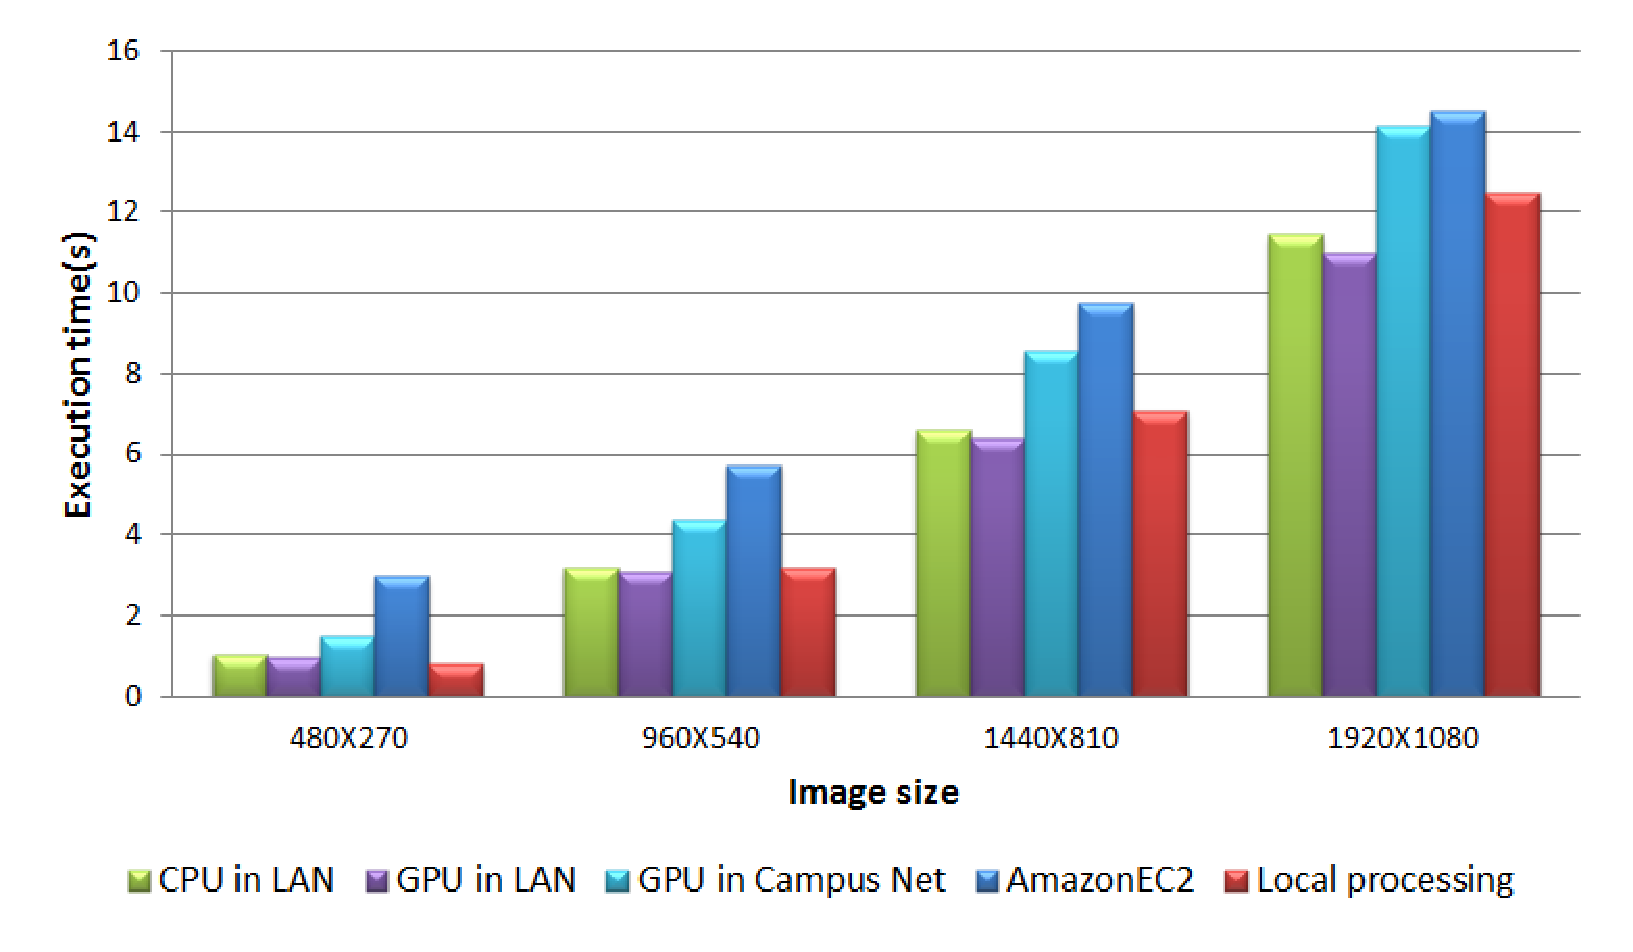
\epsfig{file=figs/time_sobelfilter.eps, width=5.0in}
\caption{Total execution time for sobelfilter with various
configurations}
\label{fig:time_sobelfilter}
\end{figure}
%
\begin{figure}
\centering
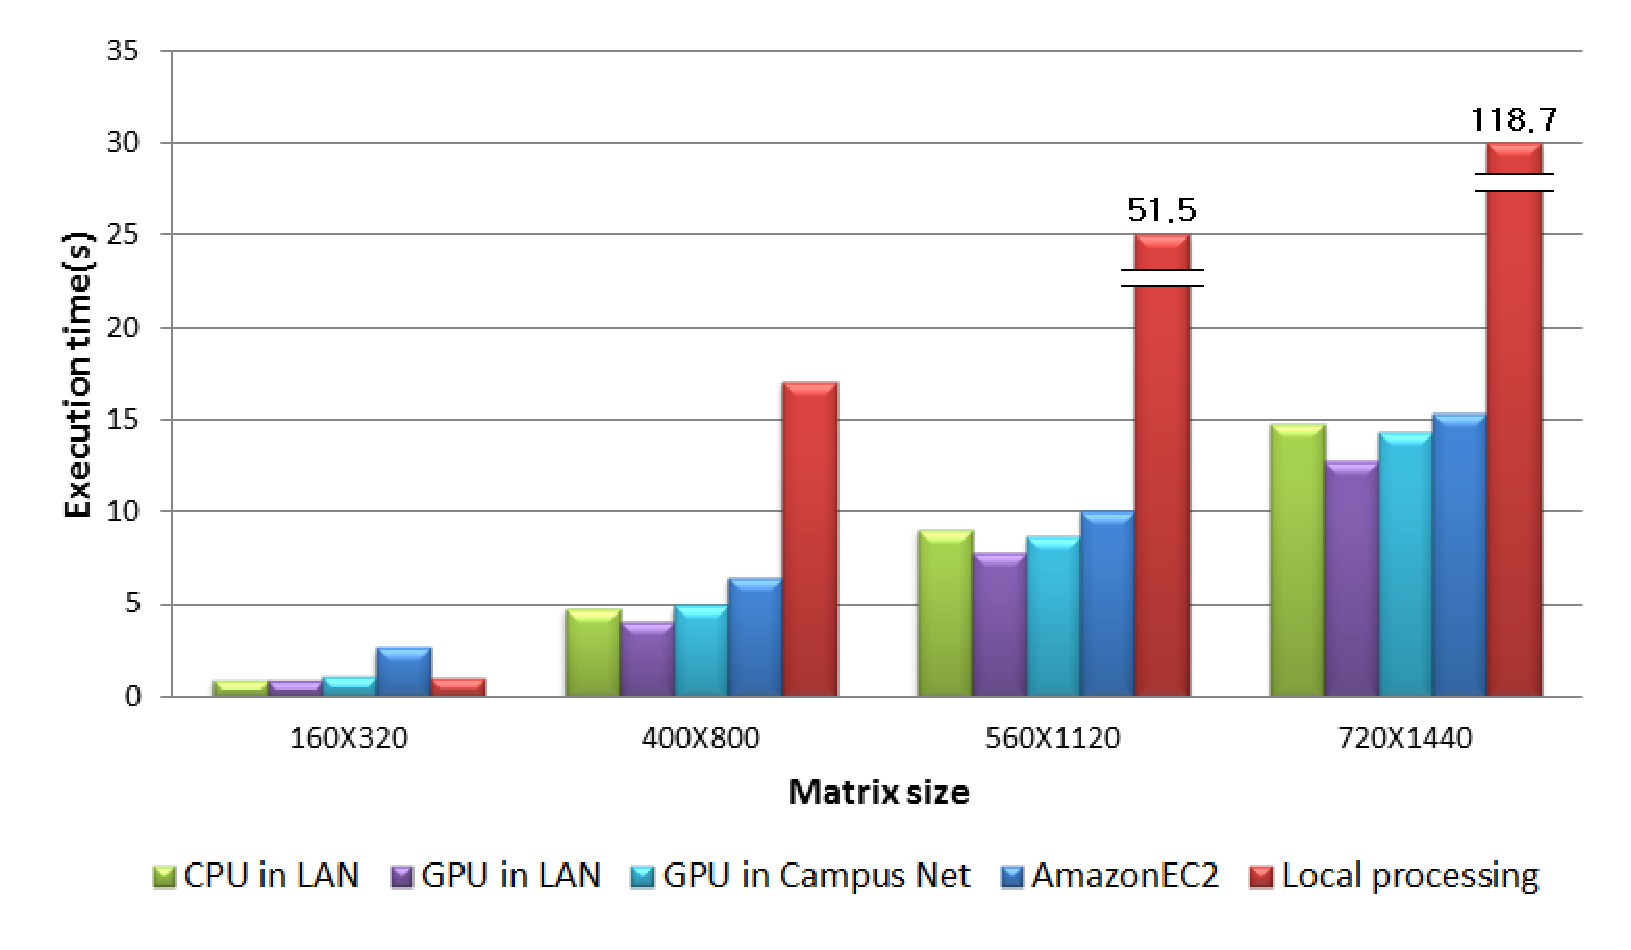
\epsfig{file=figs/time_matrix.eps, width=5.0in}
\caption{Total execution time for matrix multiplication with various
configurations}
\label{fig:time_matrix}
\end{figure}
%
\begin{figure}
\centering
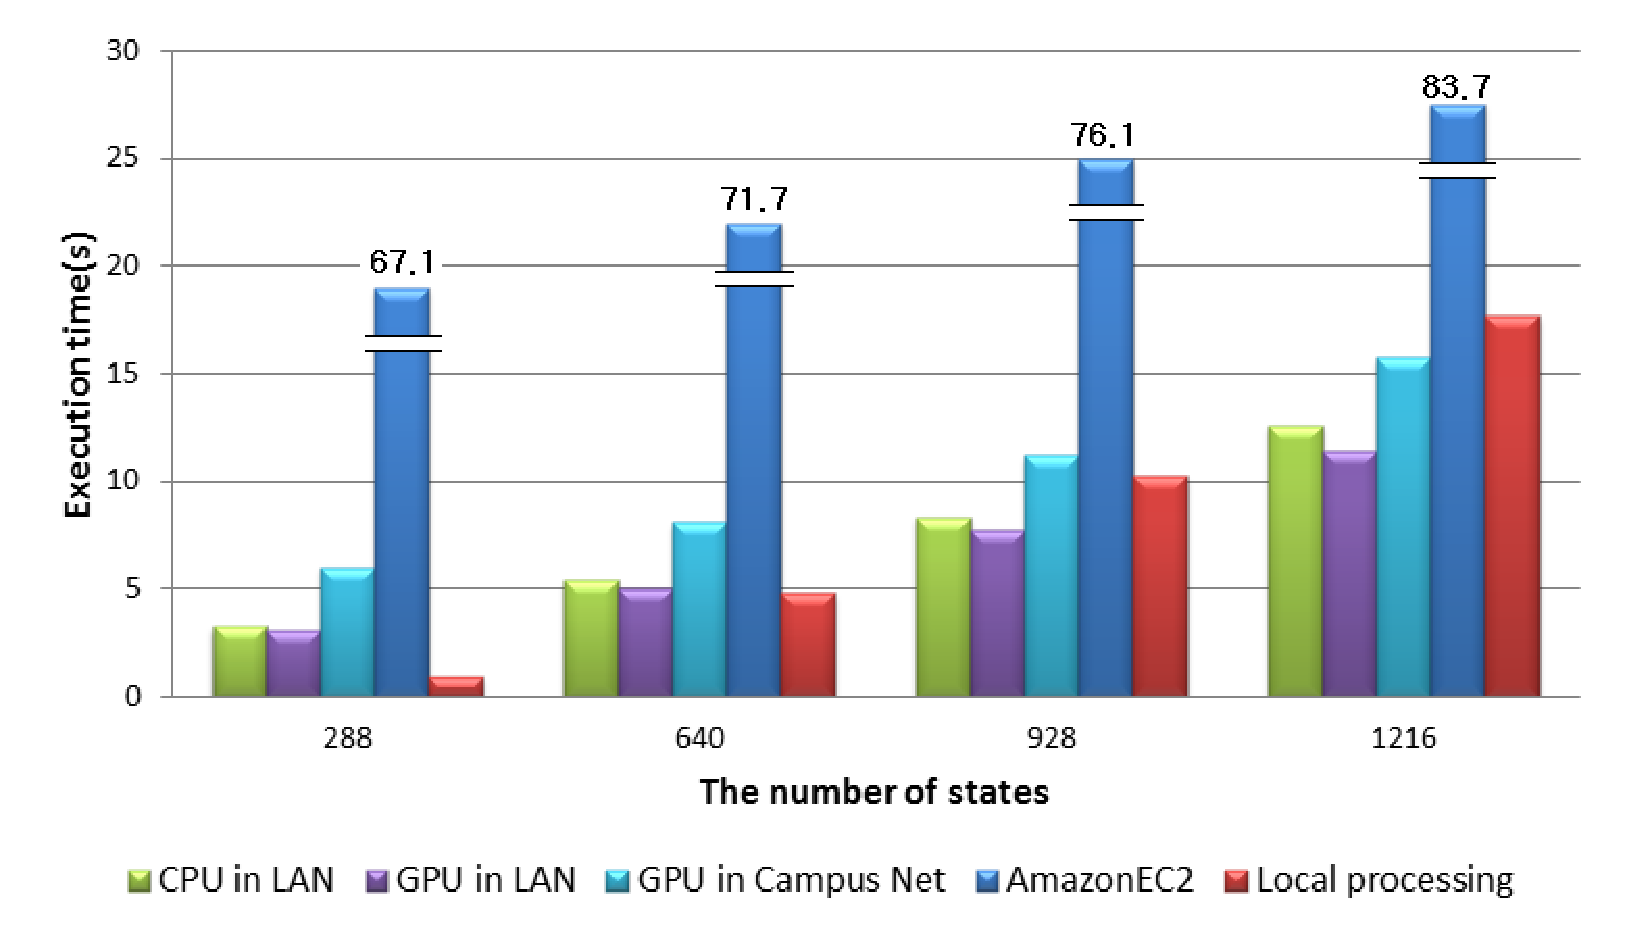
\epsfig{file=figs/time_hmm.eps, width=5.0in}
\caption{Total execution time for hidden Markov model with various
configurations}
\label{fig:time_hmm}
\end{figure}
%
\begin{figure}
\centering
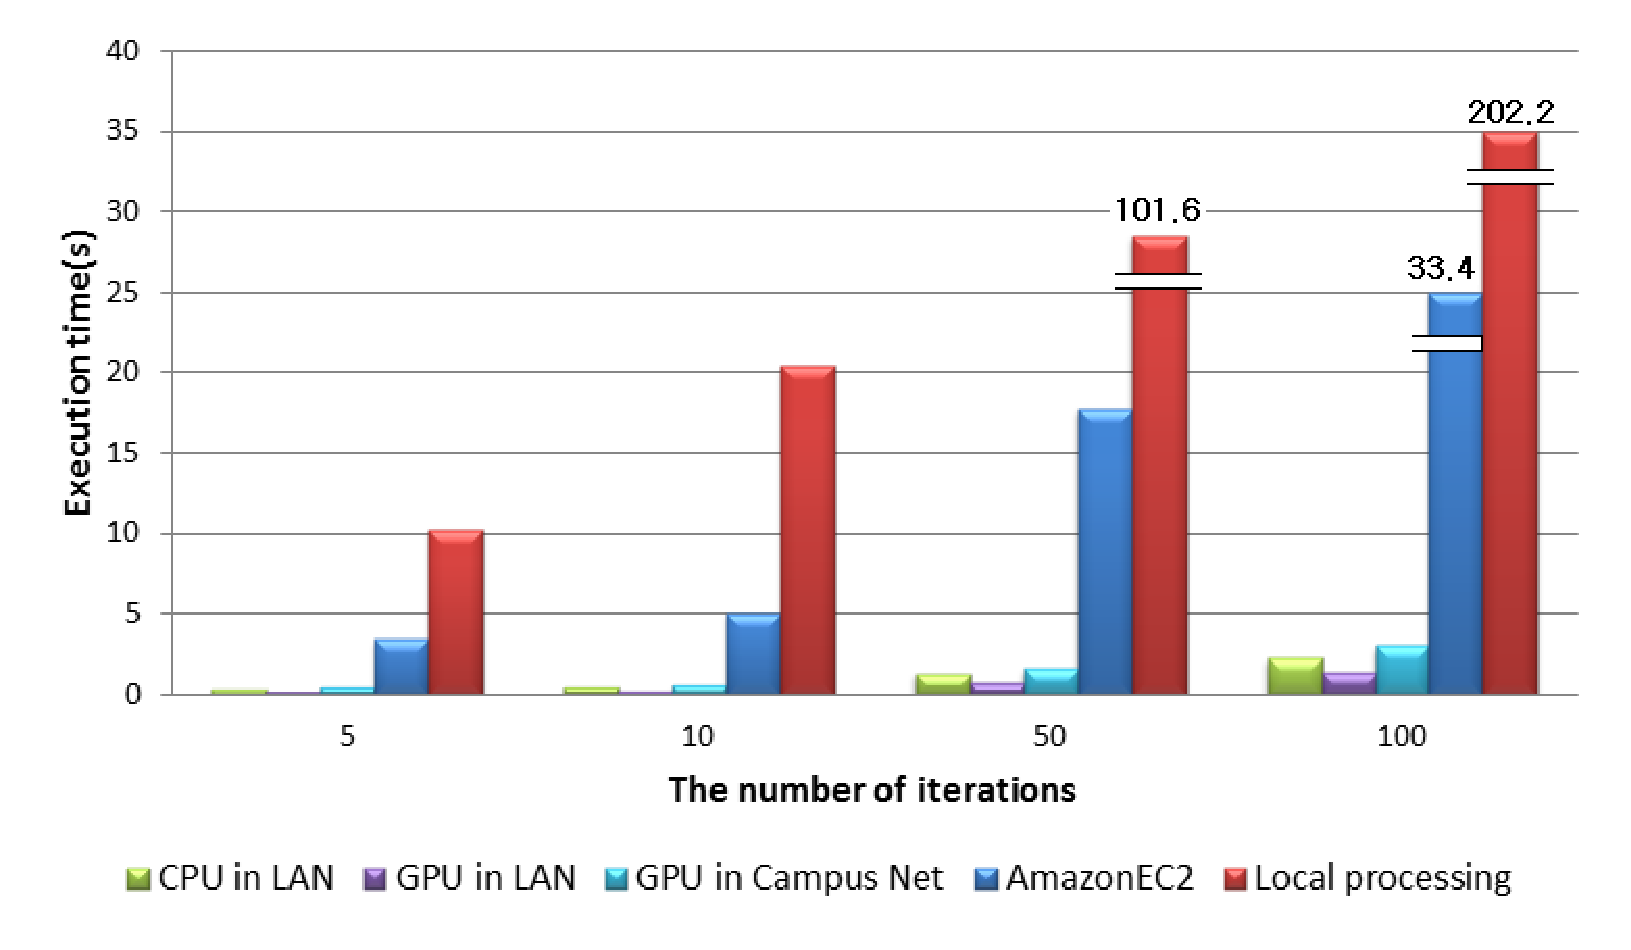
\epsfig{file=figs/time_nbody.eps, width=5.0in}
\caption{Total execution time for {\it N}-body physics with various
configurations}
\label{fig:time_nbody}
\end{figure}
%
\subsection{Energy Consumption}
\label{character:energy}
%
\begin{figure}
\centering
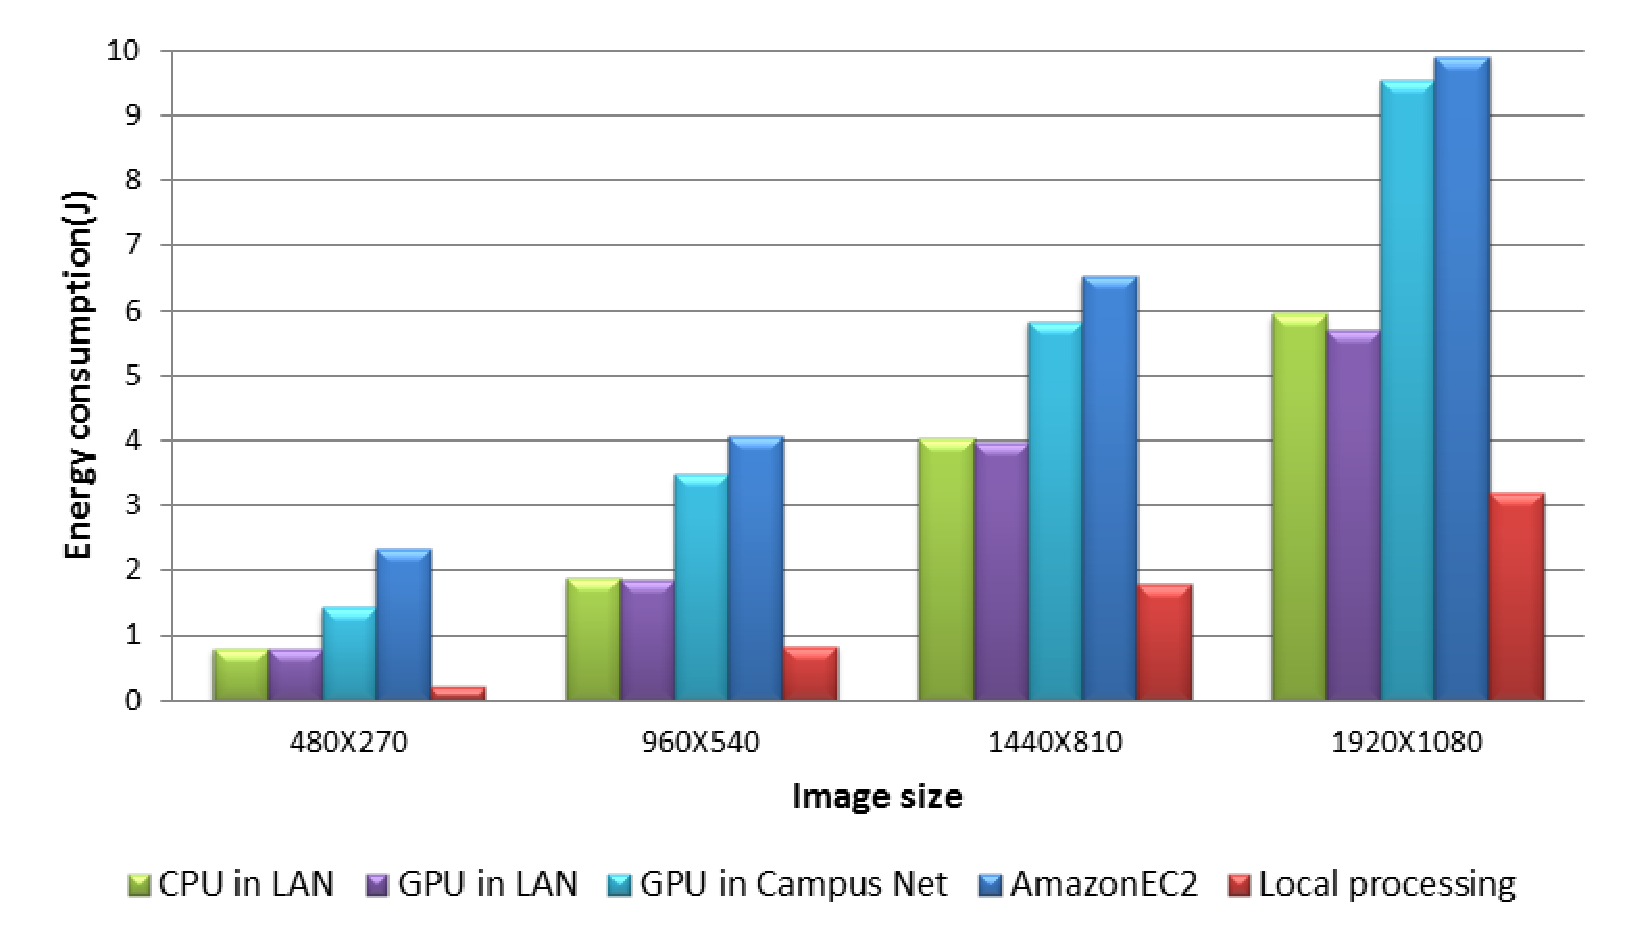
\epsfig{file=figs/energy_sobelfilter.eps, width=5.0in}
\caption{Energy consumption for sobelfilter with various configurations}
\label{fig:energy_sobelfilter}
\end{figure}
%
\begin{figure}
\centering
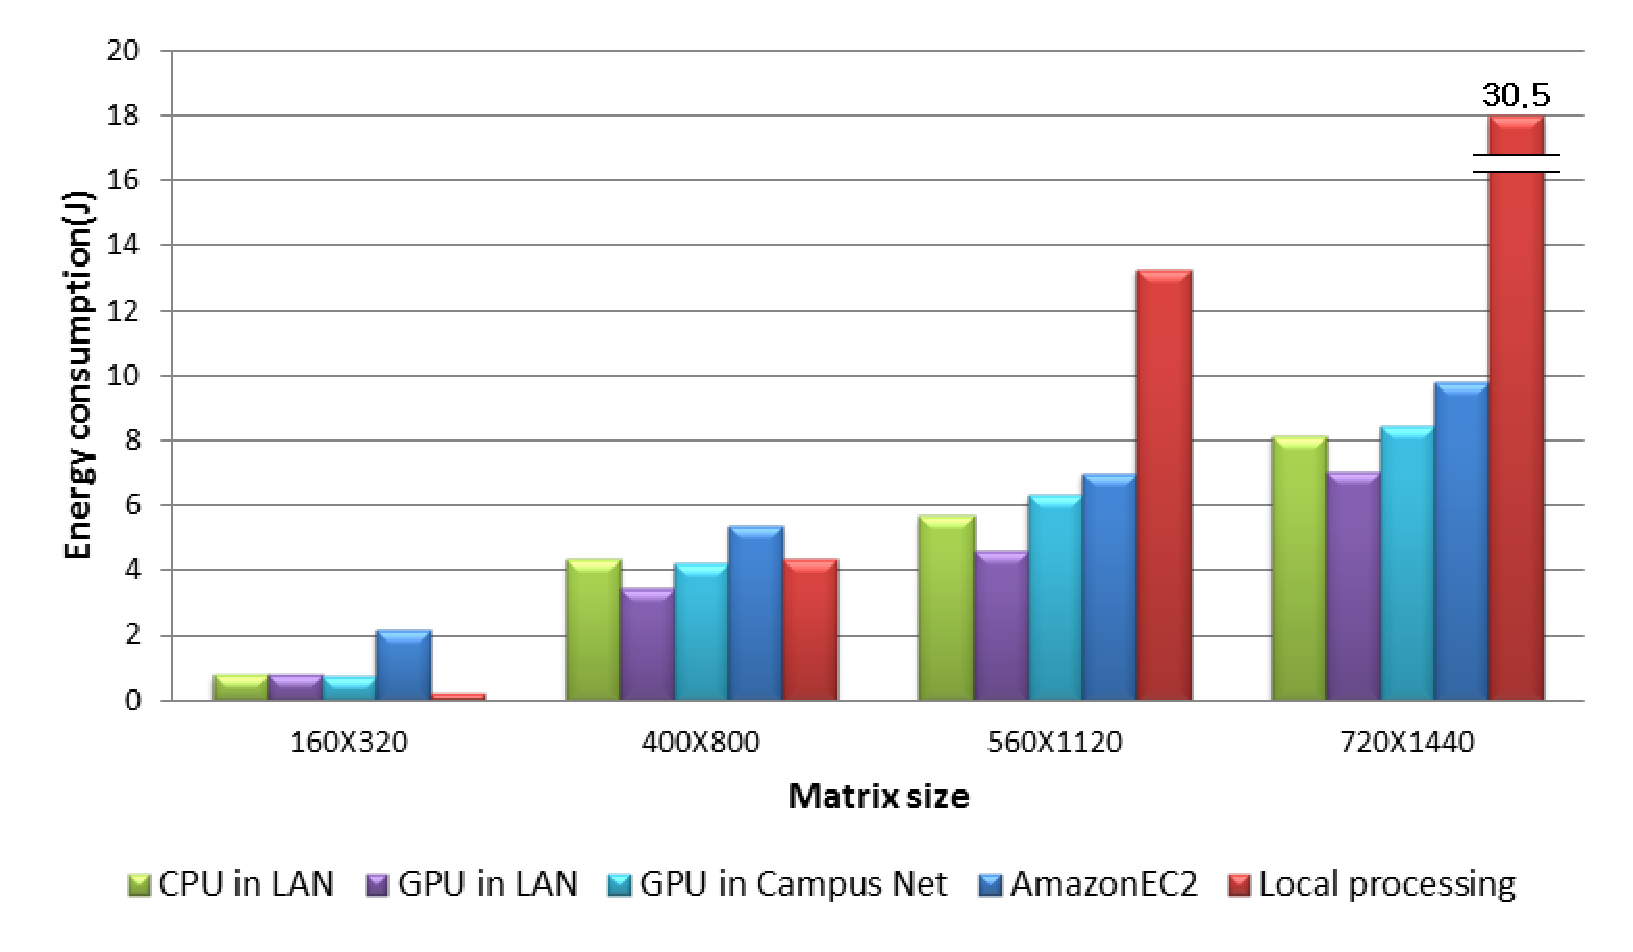
\epsfig{file=figs/energy_matrix.eps, width=5.0in}
\caption{Energy consumption for matrix multiplication with various
configurations}
\label{fig:energy_matrix}
\end{figure}
%
\begin{figure}
\centering
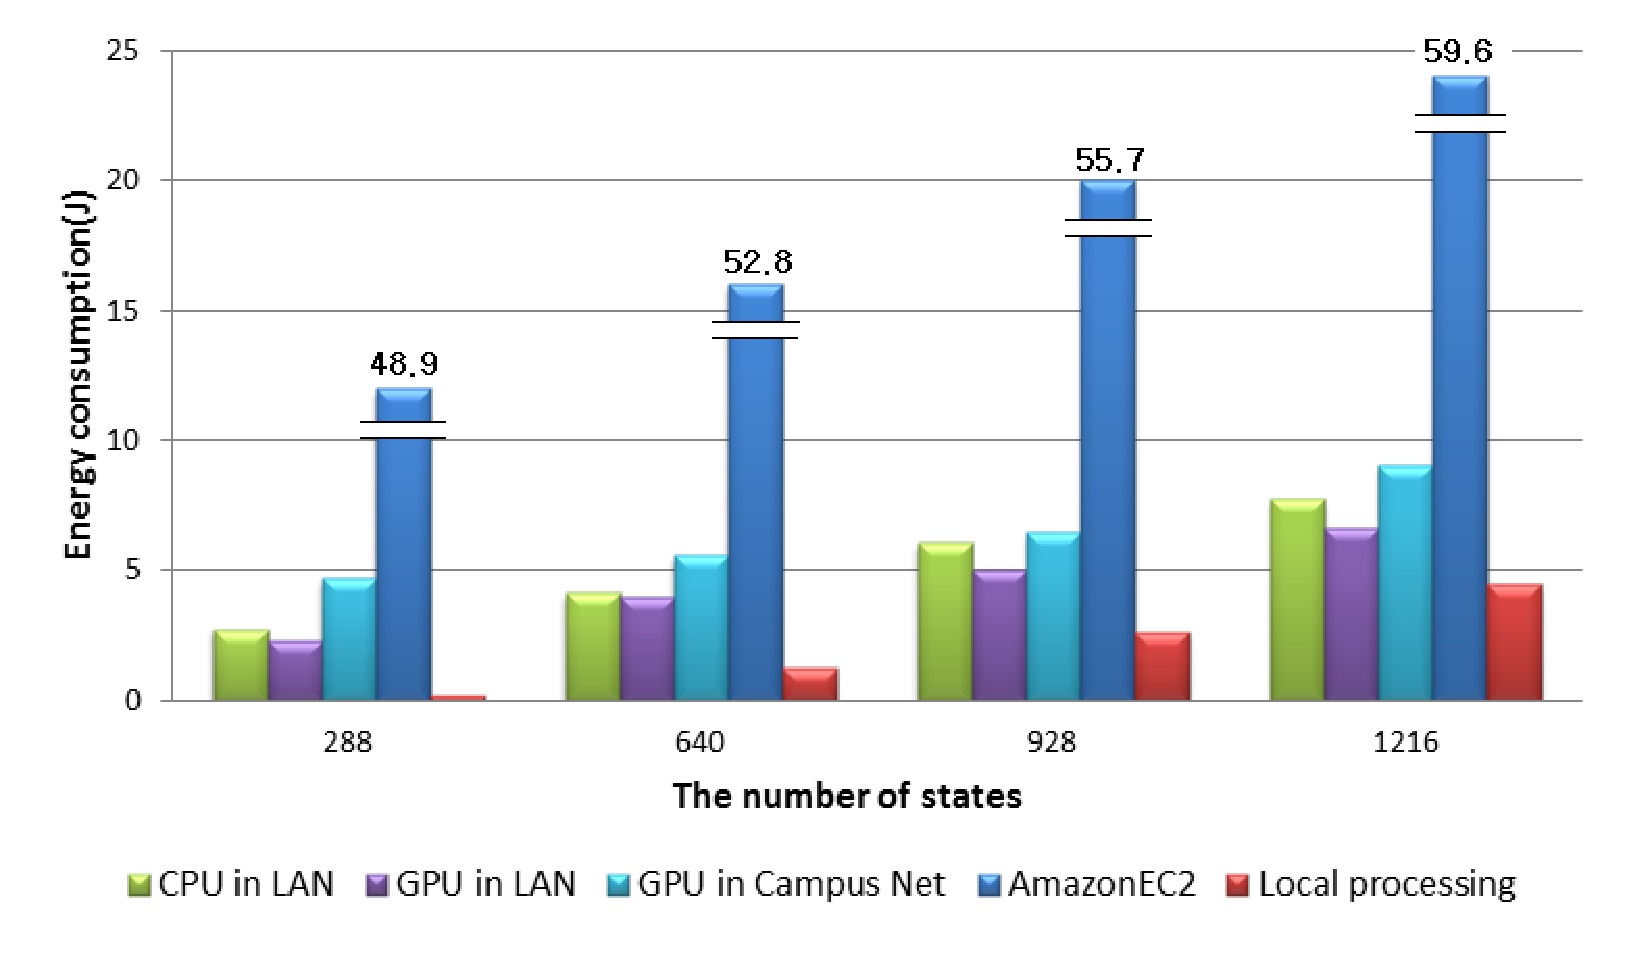
\epsfig{file=figs/energy_hmm.eps, width=5.0in}
\caption{Energy consumption for hidden Markov model with various
configurations}
\label{fig:energy_hmm}
\end{figure}
%
\begin{figure}
\centering
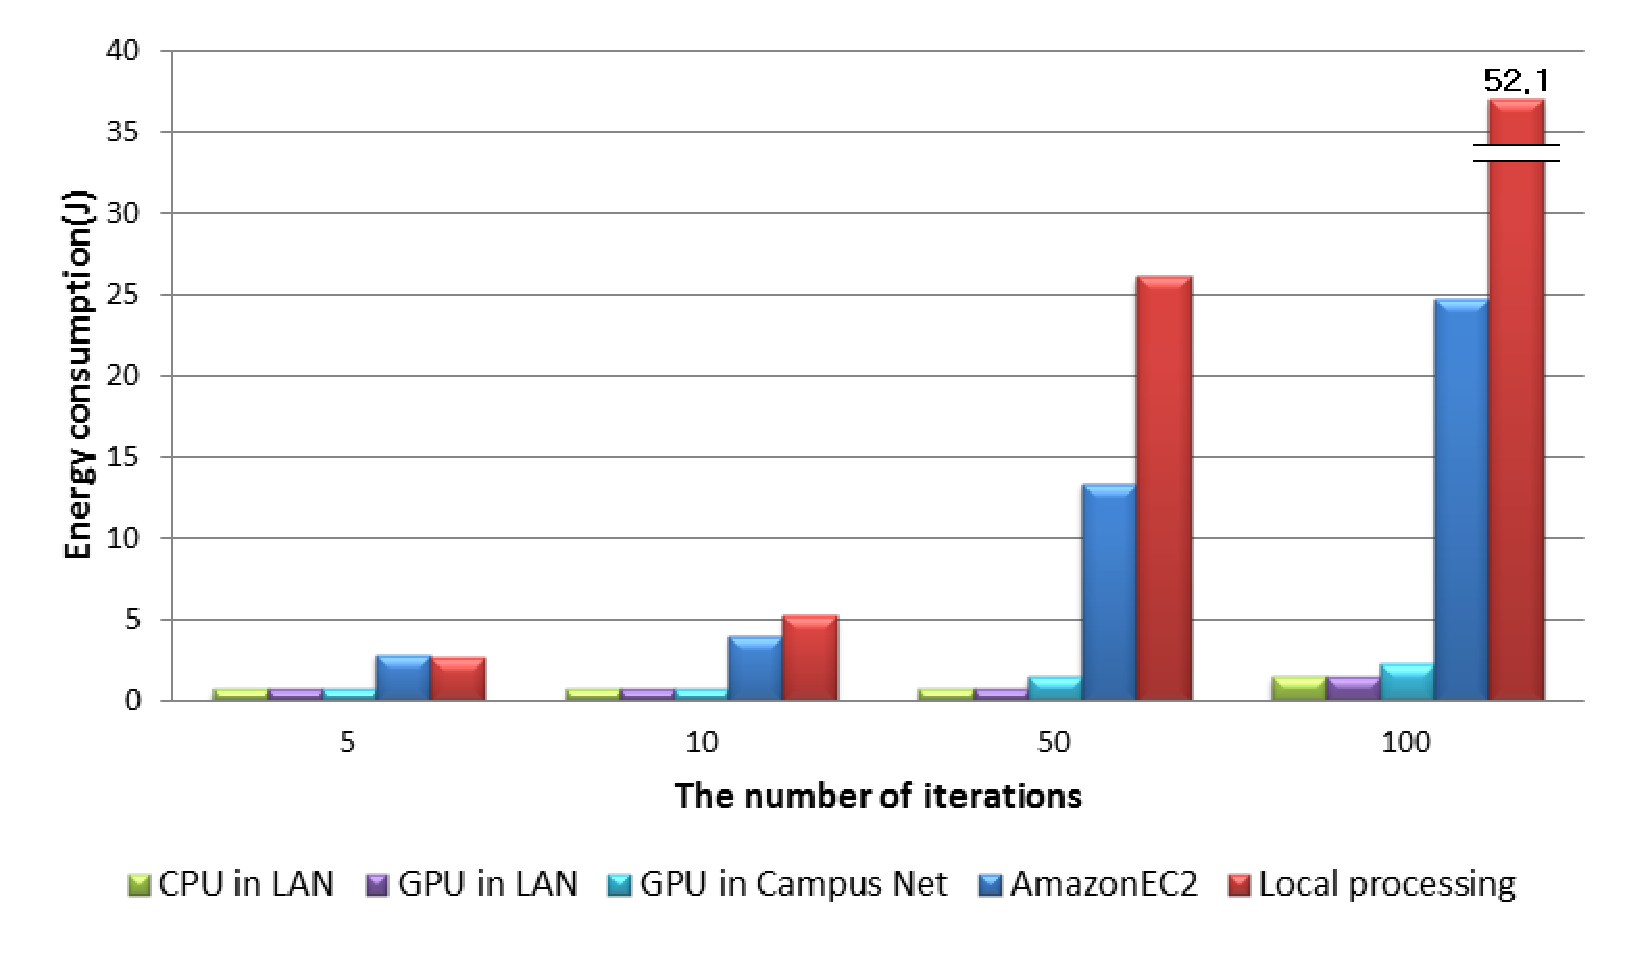
\epsfig{file=figs/energy_nbody.eps, width=5.0in}
\caption{Energy consumption for {\it N}-body physics with various configurations}
\label{fig:energy_nbody}
\end{figure}
%
To profile energy consumption of the mobile device, I used
PowerTutor~\cite{powertutor} which is an application for the variants of Android
devices that displays the power consumed by major components such as
GPU, network interfaces, LCD display, and GPS receiver.\\ 
%
A similar pattern for energy consumption of the mobile device as
the execution time is shown in
Figure~\ref{fig:energy_sobelfilter},~\ref{fig:energy_matrix},~\ref{fig:energy_hmm},
and~\ref{fig:energy_nbody}.
%
As computation to communication value is higher, 
it is likely that offloading is more beneficial than local processing.
%
However, it is worth noting that though some cases for sobelfilter
showed the benefits from offloading in terms of the execution time,
offloading consumes more than local processing as shown in Figure
3(a).
%
This dissimilar result comes from the discrepancy in the amount of power
consumed by CPU and the WiFi networking card.
%
According to the measurement data profiled by PowerTutor, CPU consumes
200$\sim$220{\it mW} per second in active mode, while the
WiFi networking card consumes about 710$\sim$720{\it mW}
per second in high power mode.
%
For that reason, even though offloading is faster than local processing,
it is possible that offloading consumes more energy than local
processing.
%
However, in matrix multiplication and {\it N}-body physics which
result in extremely high speed-up by offloading, it is observed that
offloading also improves energy implication as shown in
Figure~\ref{fig:energy_matrix} and~\ref{fig:energy_nbody}. 
%
\section{Summary}
\label{character:summary}
%
In this section, I analyzed the behavior of the mobile offloading
framework in terms of the offloading performance and energy implication
of the mobile devices with respect to characteristics of workloads and
environmental factors such as network conditions or the computing
capabilities of remote resources.
%
In order to characterize the workloads, I used computation to
communication ratio calculated by the local processing time divided by
the time for data transfer.
%
Furthermore, as part of the workload characterization effort, I
developed the OpenCL-based remote offloading framework by broadening the
scope of heterogeneity to include a new kind of platform component: the
computing capabilities on remote resources. 
%
I accomplish this by extending the well-defined hardware-level
offloading standard, OpenCL framework to support the various range of
remote computing elements over the network using the regular TCP/IP
network stack.
%
Also, I configured both local and wide area networks in which the
various computing capabilities are deployed to evaluate the impact of
environmental factors into the offloading performance.\\
%
According to the analysis, the benefits and the costs of the remote
offloading depend on computation to communication ratio as well as the
programming flow related to how the client and the server interact each
other.
%
In fact, as computation to communication ratio becomes higher, 
the performance improvement and the conservation of energy consumption 
also increase.
%
Moreover, in the cases of hidden Markov model and {\it N}-body
physics, I observed that the programming flow is also important to
analyze the behavior of the remote offloading for the mobile
platforms.  
%
I believe that the numerical results presented in this section guides the basis
of designing the intelligent runtime offloading scheduler which is
described in next section.
